\documentclass{anstrans}
%%%%%%%%%%%%%%%%%%%%%%%%%%%%%%%%%%%
\title{FUEL CYCLE PERFORMANCE OF FAST SPECTRUM \\
  MOLTEN SALT REACTOR DESIGNS}
\author{Andrei Rykhlevskii,$^{*}$ Benjamin R. Betzler,$^{\dagger}$ Andrew Worrall,$^{\dagger}$ and Kathryn Huff,$^{*}$}

\institute{
$^{*}$Dept. of Nuclear, Plasma, and Radiological Engineering, University of Illinois at 
  Urbana-Champaign, Urbana, IL \\ andreir2@illinois.edu
\and
$^{\dagger}$Oak Ridge National Laboratory, 1 Bethel Valley Road, Oak Ridge, TN, USA
}

%%%% packages and definitions (optional)
\usepackage{graphicx} % allows inclusion of graphics
\usepackage{booktabs} % nice rules (thick lines) for tables
\usepackage{microtype} % improves typography for PDF
\usepackage[acronym,toc]{glossaries}
%\newacronym{<++>}{<++>}{<++>}
\newacronym[longplural={metric tons of heavy metal}]{MTHM}{MTHM}{metric ton of heavy metal}
\newacronym{ABM}{ABM}{agent-based modeling}
\newacronym{ACDIS}{ACDIS}{Program in Arms Control \& Domestic and International Security}
\newacronym{AHTR}{AHTR}{Advanced High Temperature Reactor}
\newacronym{ANDRA}{ANDRA}{Agence Nationale pour la gestion des D\'echets RAdioactifs, the French National Agency for Radioactive Waste Management}
\newacronym{ANL}{ANL}{Argonne National Laboratory}
\newacronym{ANS}{ANS}{American Nuclear Society}
\newacronym{API}{API}{application programming interface}
\newacronym{ARE}{ARE}{Aircraft Reactor Experiment}
\newacronym{ARFC}{ARFC}{Advanced Reactors and Fuel Cycles}
\newacronym{ASME}{ASME}{American Society of Mechanical Engineers}
\newacronym{ATWS}{ATWS}{Anticipated Transient Without Scram}
\newacronym{BDBE}{BDBE}{Beyond Design Basis Event}
\newacronym{BIDS}{BIDS}{Berkeley Institute for Data Science}
\newacronym{CAFCA}{CAFCA}{ Code for Advanced Fuel Cycles Assessment }
\newacronym{CDTN}{CDTN}{Centro de Desenvolvimento da Tecnologia Nuclear}
\newacronym{CFD}{CFD}{Computational Fluid Dynamics}
\newacronym{CEA}{CEA}{Commissariat \`a l'\'Energie Atomique et aux \'Energies Alternatives}
\newacronym{CI}{CI}{continuous integration}
\newacronym{CNEN}{CNEN}{Comiss\~{a}o Nacional de Energia Nuclear}
\newacronym{CNERG}{CNERG}{Computational Nuclear Engineering Research Group}
\newacronym{COSI}{COSI}{Commelini-Sicard}
\newacronym{COTS}{COTS}{commercial, off-the-shelf}
\newacronym{CR}{CR}{conversion ratio}
\newacronym{CSNF}{CSNF}{commercial spent nuclear fuel}
\newacronym{CTAH}{CTAHs}{Coiled Tube Air Heaters}
\newacronym{CUBIT}{CUBIT}{CUBIT Geometry and Mesh Generation Toolkit}
\newacronym{CURIE}{CURIE}{Centralized Used Fuel Resource for Information Exchange}
\newacronym{DAG}{DAG}{directed acyclic graph}
\newacronym{DANESS}{DANESS}{Dynamic Analysis of Nuclear Energy System Strategies}
\newacronym{DBE}{DBE}{Design Basis Event}
\newacronym{DESAE}{DESAE}{Dynamic Analysis of Nuclear Energy Systems Strategies}
\newacronym{DHS}{DHS}{Department of Homeland Security}
\newacronym{DOE}{DOE}{Department of Energy}
\newacronym{DRACS}{DRACS}{Direct Reactor Auxiliary Cooling System}
\newacronym{DRE}{DRE}{dynamic resource exchange}
\newacronym{DSNF}{DSNF}{DOE spent nuclear fuel}
\newacronym{DU}{DU}{depleted uranium}
\newacronym{DYMOND}{DYMOND}{Dynamic Model of Nuclear Development }
\newacronym{EBS}{EBS}{Engineered Barrier System}
\newacronym{EDF}{EDF}{Électricité de France}
\newacronym{EDZ}{EDZ}{Excavation Disturbed Zone}
\newacronym{EIA}{EIA}{U.S. Energy Information Administration}
\newacronym{EPA}{EPA}{Environmental Protection Agency}
\newacronym{EPR}{EPR}{European Pressurized Reactors}
\newacronym{EP}{EP}{Engineering Physics}
\newacronym{EU}{EU}{European Union}
\newacronym{FCO}{FCO}{Fuel Cycle Options}
\newacronym{FCT}{FCT}{Fuel Cycle Technology}
\newacronym{FEHM}{FEHM}{Finite Element Heat and Mass Transfer}
\newacronym{FEPs}{FEPs}{Features, Events, and Processes}
\newacronym{FHR}{FHR}{Fluoride-Salt-Cooled High-Temperature Reactor}
\newacronym{FLiBe}{FLiBe}{Fluoride-Lithium-Beryllium}
\newacronym{FP}{FP}{Fission Product}
\newacronym{GDSE}{GDSE}{Generic Disposal System Environment}
\newacronym{GDSM}{GDSM}{Generic Disposal System Model}
\newacronym{GENIUSv1}{GENIUSv1}{Global Evaluation of Nuclear Infrastructure Utilization Scenarios, Version 1}
\newacronym{GENIUSv2}{GENIUSv2}{Global Evaluation of Nuclear Infrastructure Utilization Scenarios, Version 2}
\newacronym{GENIUS}{GENIUS}{Global Evaluation of Nuclear Infrastructure Utilization Scenarios}
\newacronym{GIF}{GIF}{Generation IV International Forum}
\newacronym{GPAM}{GPAM}{Generic Performance Assessment Model}
\newacronym{GRSAC}{GRSAC}{Graphite Reactor Severe Accident Code}
\newacronym{GUI}{GUI}{graphical user interface}
\newacronym{HLW}{HLW}{high level waste}
\newacronym{HPC}{HPC}{high-performance computing}
\newacronym{HTC}{HTC}{high-throughput computing}
\newacronym{HTGR}{HTGR}{High Temperature Gas-Cooled Reactor}
\newacronym{IAEA}{IAEA}{International Atomic Energy Agency}
\newacronym{IEMA}{IEMA}{Illinois Emergency Mangament Agency}
\newacronym{IHLRWM}{IHLRWM}{International High Level Radioactive Waste Management}
\newacronym{INL}{INL}{Idaho National Laboratory}
\newacronym{IPRR1}{IRP-R1}{Instituto de Pesquisas Radioativas Reator 1}
\newacronym{IRP}{IRP}{Integrated Research Project}
\newacronym{ISFSI}{ISFSI}{Independent Spent Fuel Storage Installation}
\newacronym{ISRG}{ISRG}{Independent Student Research Group}
\newacronym{JFNK}{JFNK}{Jacobian-Free Newton Krylov}
\newacronym{LANL}{LANL}{Los Alamos National Laboratory}
\newacronym{LBNL}{LBNL}{Lawrence Berkeley National Laboratory}
\newacronym{LCOE}{LCOE}{levelized cost of electricity}
\newacronym{LDRD}{LDRD}{laboratory directed research and development}
\newacronym{LFR}{LFR}{Lead-Cooled Fast Reactor}
\newacronym{LLNL}{LLNL}{Lawrence Livermore National Laboratory}
\newacronym{LMFBR}{LMFBR}{Liquid Metal Fast Breeder Reactor}
\newacronym{LOFC}{LOFC}{Loss of Forced Cooling}
\newacronym{LOHS}{LOHS}{Loss of Heat Sink}
\newacronym{LOLA}{LOLA}{Loss of Large Area}
\newacronym{LP}{LP}{linear program}
\newacronym{LWR}{LWR}{light water reactor}
\newacronym{MAGNOX}{MAGNOX}{Magnesium Alloy Graphie Moderated Gas Cooled Uranium Oxide Reactor}
\newacronym{MA}{MA}{minor actinide}
\newacronym{MCNP}{MCNP}{Monte Carlo N-Particle code}
\newacronym{MILP}{MILP}{mixed-integer linear program}
\newacronym{MIT}{MIT}{the Massachusetts Institute of Technology}
\newacronym{MOAB}{MOAB}{Mesh-Oriented datABase}
\newacronym{MOOSE}{MOOSE}{Multiphysics Object-Oriented Simulation Environment}
\newacronym{MOSART}{MOSART}{Molten Salt Actinide Recycler and Transmuter}
\newacronym{MOX}{MOX}{mixed oxide}
\newacronym{MPI}{MPI}{Message Passing Interface}
\newacronym{MCSFR}{MCSFR}{Molten Chloride Salt Fast Reactor}
\newacronym{MSBR}{MSBR}{Molten Salt Breeder Reactor}
\newacronym{MSFR}{MSFR}{Molten Salt Fast Reactor}
\newacronym{MSRE}{MSRE}{Molten Salt Reactor Experiment}
\newacronym{MSR}{MSR}{Molten Salt Reactor}
\newacronym{MT}{MT}{metric ton}
\newacronym{NAGRA}{NAGRA}{National Cooperative for the Disposal of Radioactive Waste}
\newacronym{NEAMS}{NEAMS}{Nuclear Engineering Advanced Modeling and Simulation}
\newacronym{NEUP}{NEUP}{Nuclear Energy University Programs}
\newacronym{NFCSim}{NFCSim}{Nuclear Fuel Cycle Simulator}
\newacronym{NGNP}{NGNP}{Next Generation Nuclear Plant}
\newacronym{NMWPC}{NMWPC}{Nuclear MW Per Capita}
\newacronym{NNSA}{NNSA}{National Nuclear Security Administration}
\newacronym{NPP}{NPP}{Nuclear Power Plant}
\newacronym{NPRE}{NPRE}{Department of Nuclear, Plasma, and Radiological Engineering}
\newacronym{NQA1}{NQA-1}{Nuclear Quality Assurance - 1}
\newacronym{NRC}{NRC}{Nuclear Regulatory Commission}
\newacronym{NSF}{NSF}{National Science Foundation}
\newacronym{NSSC}{NSSC}{Nuclear Science and Security Consortium}
\newacronym{NUWASTE}{NUWASTE}{Nuclear Waste Assessment System for Technical Evaluation}
\newacronym{NWF}{NWF}{Nuclear Waste Fund}
\newacronym{NWTRB}{NWTRB}{Nuclear Waste Technical Review Board}
\newacronym{OCRWM}{OCRWM}{Office of Civilian Radioactive Waste Management}
\newacronym{ORION}{ORION}{ORION}
\newacronym{ORNL}{ORNL}{Oak Ridge National Laboratory}
\newacronym{PARCS}{PARCS}{Purdue Advanced Reactor Core Simulator}
\newacronym{PBAHTR}{PB-AHTR}{Pebble Bed Advanced High Temperature Reactor}
\newacronym{PBFHR}{PB-FHR}{Pebble-Bed Fluoride-Salt-Cooled High-Temperature Reactor}
\newacronym{PEI}{PEI}{Peak Environmental Impact}
\newacronym{PH}{PRONGHORN}{PRONGHORN}
\newacronym{PRIS}{PRIS}{Power Reactor Information System}
\newacronym{PRKE}{PRKE}{Point Reactor Kinetics Equations}
\newacronym{PSPG}{PSPG}{Pressure-Stabilizing/Petrov-Galerkin}
\newacronym{PWAR}{PWAR}{Pratt and Whitney Aircraft Reactor}
\newacronym{PWR}{PWR}{Pressurized Water Reactor}
\newacronym{PyNE}{PyNE}{Python toolkit for Nuclear Engineering}
\newacronym{PyRK}{PyRK}{Python for Reactor Kinetics}
\newacronym{QA}{QA}{quality assurance}
\newacronym{RDD}{RD\&D}{Research Development and Demonstration}
\newacronym{RD}{R\&D}{Research and Development}
\newacronym{REE}{REE}{rare earth element}
\newacronym{RELAP}{RELAP}{Reactor Excursion and Leak Analysis Program}
\newacronym{RIA}{RIA}{Reactivity Insertion Accident}
\newacronym{RIF}{RIF}{Region-Institution-Facility}
\newacronym{RTh}{RTh}{recovered thorium}
\newacronym{RU}{RU}{recovered uranium}
\newacronym{SFR}{SFR}{Sodium-Cooled Fast Reactor}
\newacronym{SINDAG}{SINDA{\textbackslash}G}{Systems Improved Numerical Differencing Analyzer $\backslash$ Gaski}
\newacronym{SKB}{SKB}{Svensk K\"{a}rnbr\"{a}nslehantering AB}
\newacronym{SNF}{SNF}{spent nuclear fuel}
\newacronym{SNL}{SNL}{Sandia National Laboratory}
\newacronym{STC}{STC}{specific temperature change}
\newacronym{SUPG}{SUPG}{Streamline-Upwind/Petrov-Galerkin}
\newacronym{SWF}{SWF}{Separations and Waste Forms}
\newacronym{SWU}{SWU}{Separative Work Unit}
\newacronym{TRIGA}{TRIGA}{Training Research Isotope General Atomic}
\newacronym{TRISO}{TRISO}{Tristructural Isotropic}
\newacronym{TRU}{TRU}{transuranic}
\newacronym{TSM}{TSM}{Total System Model}
\newacronym{TSPA}{TSPA}{Total System Performance Assessment for the Yucca Mountain License Application}
\newacronym{ThOX}{ThOX}{thorium oxide}
\newacronym{UFD}{UFD}{Used Fuel Disposition}
\newacronym{UML}{UML}{Unified Modeling Language}
\newacronym{UOX}{UOX}{uranium oxide}
\newacronym{UQ}{UQ}{uncertainty quantification}
\newacronym{US}{US}{United States}
\newacronym{UW}{UW}{University of Wisconsin}
\newacronym{VISION}{VISION}{the Verifiable Fuel Cycle Simulation Model}
\newacronym{VVER}{VVER}{Voda-Vodyanoi Energetichesky Reaktor (Russian Pressurized Water Reactor)}
\newacronym{VV}{V\&V}{verification and validation}
\newacronym{WIPP}{WIPP}{Waste Isolation Pilot Plant}
\newacronym{YMR}{YMR}{Yucca Mountain Repository Site}


\makeglossaries
\newcommand{\SN}{S$_N$}
\renewcommand{\vec}[1]{\bm{#1}} %vector is bold italic
\newcommand{\vd}{\bm{\cdot}} % slightly bold vector dot
\newcommand{\grad}{\vec{\nabla}} % gradient
\newcommand{\ud}{\mathop{}\!\mathrm{d}} % upright derivative symbol

\begin{document}
%%%%%%%%%%%%%%%%%%%%%%%%%%%%%%%%%%%%%%%%%%%%%%%%%%%%%%%%%%%%%%%%%%%%%%%%%%%%%%%%
\section{INTRODUCTION} 
\label{sec:intro}
A liquid-fueled \gls{MSR} concepts promise one of the most desirable and competitive, sustainable energy among of many advanced reactor systems \cite{siemer_why_2015}. In \gls{MSR} fissile and/or fertile materials are dissolved in carrier molten salt (e.g., LiF, NaCl) which leads to immediate advantages over traditional, solid-fueled, reactors. These include near-atmospheric pressure in the primary loop, relatively high coolant temperature, outstanding neutron economy, a high level of inherent safety,
reduced fuel preprocessing, and the ability to continuously remove fission products and add fissile and/or fertile elements without shutdown \cite{leblanc_molten_2010}. 

Historically, researchers focused on thermal spectrum \gls{MSR} concepts with solid graphite moderator.  \gls{ORNL} operated $\approx$8 MW$_{th}$ \gls{MSRE} pilot reactor from 1965 to 1969 to test approaches/materials, demonstrate fissile recycle (both $^{233}$U and $^{235}$U), and determine generic \gls{MSR} operational characteristics \cite{macpherson_molten_1985}. Obtained experience plus promising breakthrough in reprocessing technology \cite{whatley_engineering_1970} chained \gls{ORNL} attention to the simply configured, also graphite-moderated (i.e., thermal or epithermal), single-fluid \gls{MSBR} by the end of the 1960's. The primary weakness of all one-fluid thermal \gls{MSR} concepts is the fact that the hundreds tons ($\approx$300 t for \gls{MSBR} \cite{robertson_conceptual_1971}) of expensive, radiologically contaminated, neutron-damaged graphite would have to be replaced every 4-10 years, which raises significant waste and economical issues.

In contrast, consistent with \gls{GIF} sustainability and safety goals \cite{gif_generation_2015}, unmoderated (no graphite), one- or two-fluid (blanket equipped) fast spectrum \gls{MSR} concepts eventually became the EUROATOM Consortium's ``reference" \gls{MSR} \cite{noauthor_final_2015}. Other identified advantages of fast \gls{MSR} systems comparing with conventional reactors include: (1) they can operate in breeding (CR\footnote{\gls{CR} $\equiv$ fissile generated/fissile consumed: if CR$<$1 the reactor is a ``converter"; CR$\equiv$1, an ``isobreeder"; CR$>$1, a ``breeder".}$>$1) \cite{noauthor_final_2015,simmons_assessment_1974,mourogov_potentialities_2006}, fertile-free \gls{TRU} burning, or U/Th-supported \gls{TRU} burning \cite{ignatiev_progress_2007} regime; (2) they can potentially work in both $^{232}$Th/$^{233}$U and $^{238}$U/$^{239}$Pu fuel cycles (i.e., thermal \gls{MSR} supports only Th/U); (3) they can be operated in ways that would generate very little long-lived \gls{TRU} waste, and (4) they would use less natural resources (e.g., natural uranium, natural thorium) per unit energy generated. To quantitatively estimate benefits of these capabilities fuel cycle performance analysis for various fast spectrum \gls{MSR} concepts is necessary.

Much of the analysis herein uses unit cell representations of four different fast \gls{MSR} designs: 
(1) European \gls{MSFR} \cite{noauthor_final_2015}; (2) \gls{MCSFR} \cite{simmons_assessment_1974}; (3) REBUS-3700 \cite{mourogov_potentialities_2006}; (4) \gls{MOSART} \cite{ignatiev_progress_2007}. Some of these designs are two-fluid (1, 2), operate in thorium fuel cycle (1,4), or use \gls{TRU} as start-up fissile material. The concepts (2) and (3) use chloride salts\footnote{The chlorine in the \gls{MCSFR} is fully enriched in $^{37}$Cl because $^{35}$Cl (76\% abundance) is a very strong neutron poison in fast neutron energy range.} while (1) and (2) employ fluorides. This paper discusses the depletion simulation of different fast \glspl{MSR} to identify fuel cycle performance for deployment of this reactor technology.

\section{METHODS} 
\label{sec:methods}
To determine Fuel Cycle Performance parameters full-core and simplified unit cell models of four different fast spectrum \glspl{MSR} designs were created (Fig.~\ref{fig:unit_cell}).  Table~\ref{table:fsmsr_concepts} contains summary of principal data of these designs. Fuel cycle performance analysis required depletion simulation for each reactor concept over the whole system lifetime which in this work assumed 60 years\footnote{Lifetime for fast \gls{MSR} limited by neutron damage on the reactor vessel. Further R\&D activities should be performed to evaluate maximum fast neutron fluence and assess structural materials choice.}. Full-core 60-years depletion computation for \gls{MSR} model required massive computing power. Computation time can be significantly reduced by performing depletion simulation for simplified unit cell representation instead of full-core one with sophisticated geometry.
\begin{figure}[!htb]
  \centering
  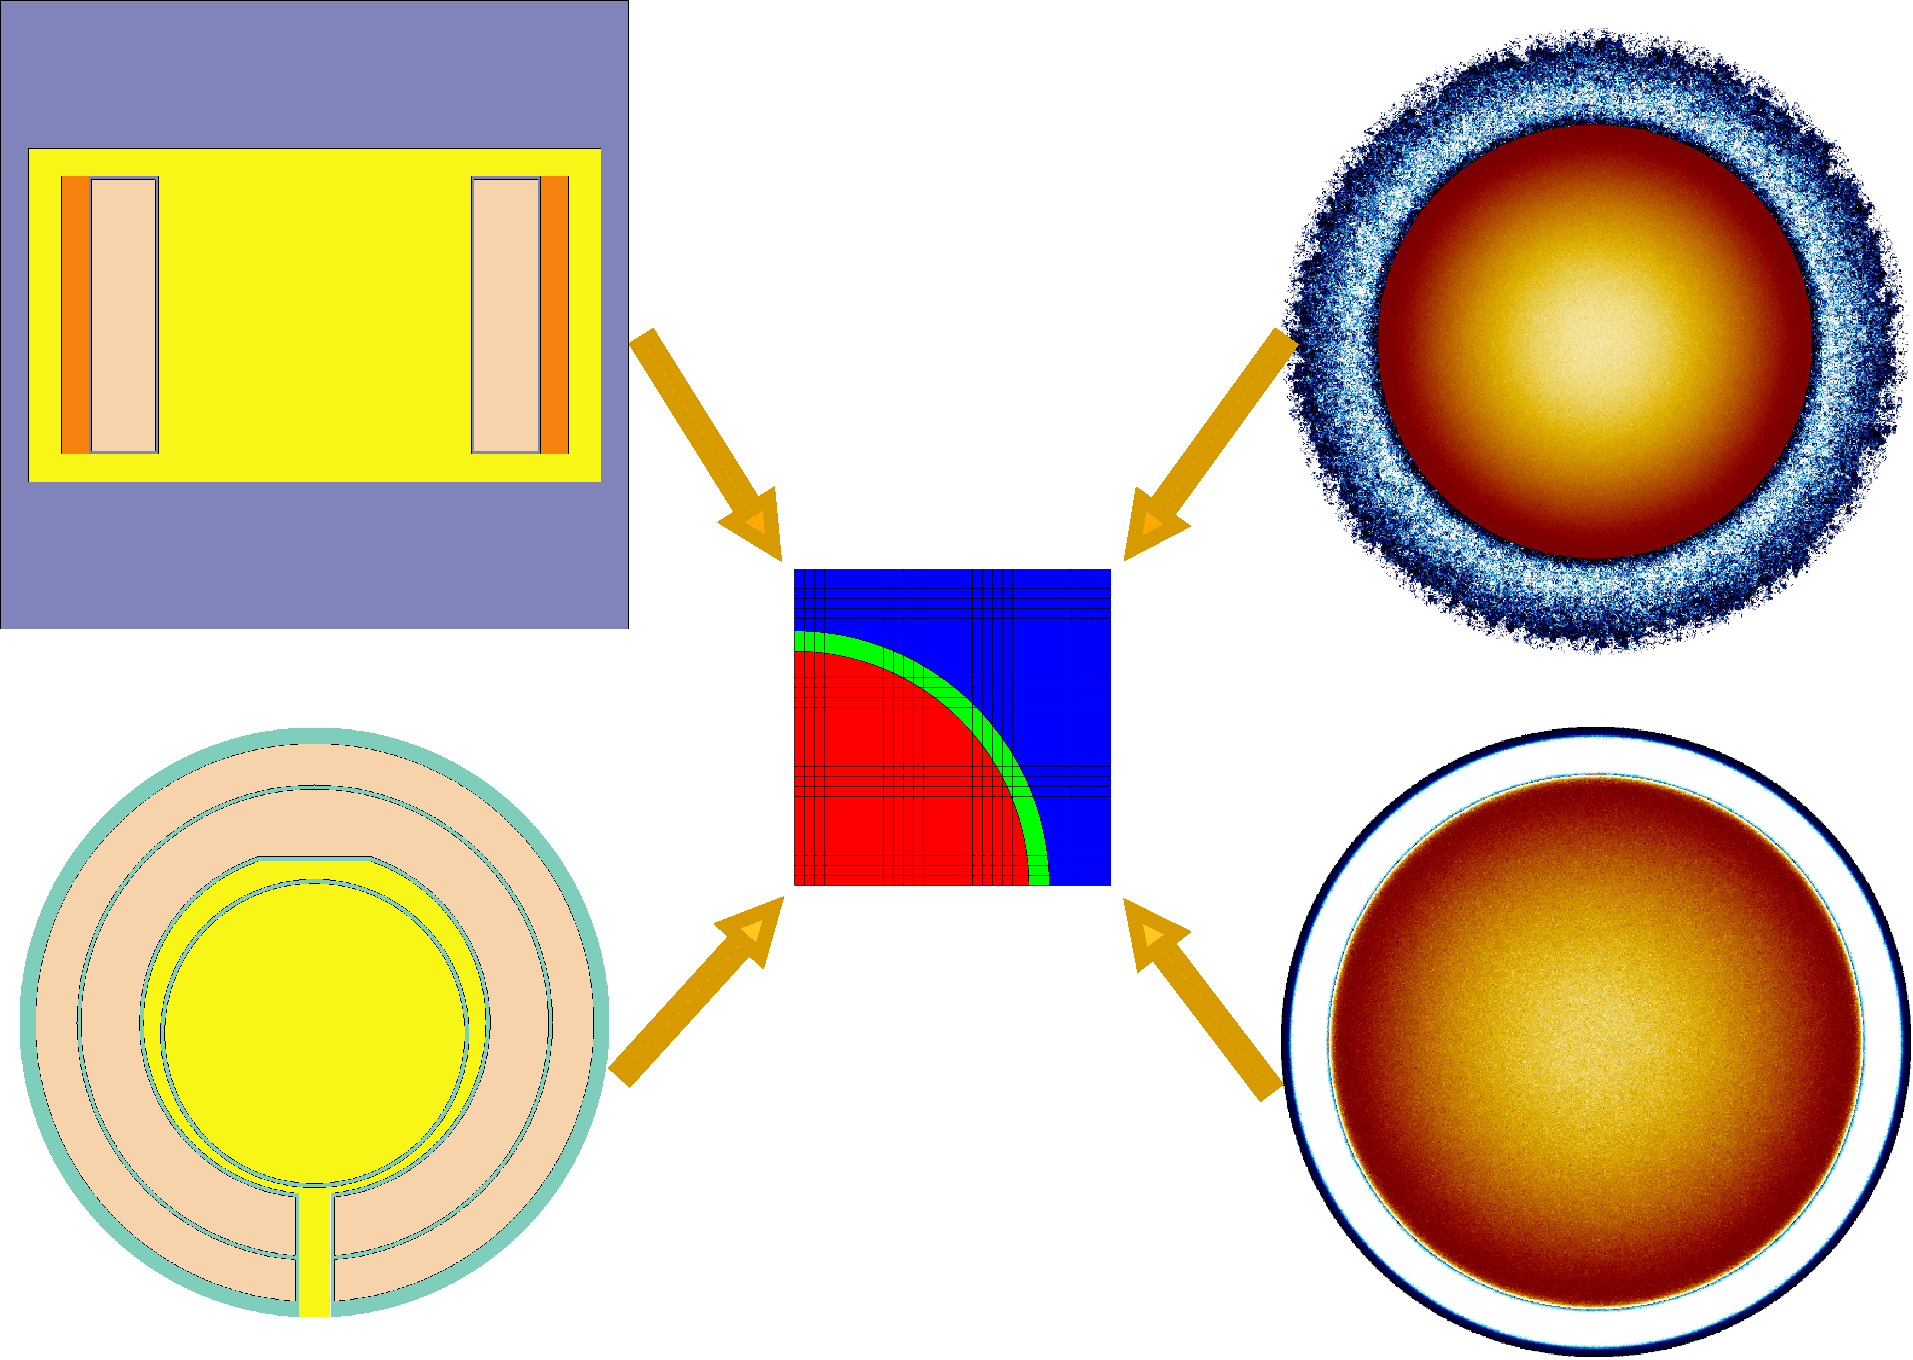
\includegraphics[scale=0.265]{./Figures/fsmsrs.pdf}
  \caption{Full-core 3D models of \gls{MSFR} (upper left), \gls{MCSFR} (lower left), REBUS-3700 (upper right), \gls{MOSART} (lower right), and 2D unit cell model (center) showing fuel salt (red), fertile salt (green), structural material (blue).}   
  \label{fig:unit_cell}
\end{figure}
\begin{table*}[!htb]
  \centering
  \caption{Principal data of selected fast spectrum \glspl{MSR} designs.}
  \label{table:fsmsr_concepts} 
  \begin{tabular}{p{0.25\textwidth} p{0.15\textwidth} p{0.18\textwidth} p{0.15\textwidth} p{0.15\textwidth}} \toprule 
   Parameter & \gls{MSFR} & \gls{MCSFR} & REBUS-3700 & \gls{MOSART} \\ \midrule
   Thermal power, MW 				&  3,000 & 6,000     & 3,700 & 2,400   \\ 
   Fuel salt volume (in/out of core)       &18 (9/9)& 38 (16/22)& 55.6 (36.9/18.7) & 49.05 (32.7/16.35) \\ 
   Fertile salt volume (in/out of blanket) & 7.3 (7.3/0) & 75 (55/22)    & --- & --- \\
   Fuel and fertile salt initial composition (mol\%) & LiF-ThF$_4$-$^{233}$UF$_4$ (77.5-19.9-2.6) LiF-ThF$_4$ \newline (77.5-22.5) & NaCl-UCl$_3$-$^{239}$PuCl$_3$ (60-36-4) \newline NaCl-UCl$_3$ \newline (60-40)    
   & 55mol\%NaCl+ 45mol\%(natU+ 16.7at.\%TRU)Cl$_3$ 
   & LiF-BeF$_2$-ThF$_4$-TRUF$_3$  \newline (69.72-27-1.28) \\
   Fuel cycle & Th/$^{233}$U & U/Pu  & U/TRU & Th/$^{233}$U \\
   Initial fissile inventory, t & \ 5.060 & \ 9.400    & 18.061 & 9.637 \\ \bottomrule 
  \end{tabular}
\end{table*}

\subsection{Models description} 
\label{sec:model}
In contrast with thermal \gls{MSR}, fast spectrum concepts do not have channel or assembly structure but contain homogenized fuel mixture in cylindrical or spherical vessel. Two-fluid systems also have cylindrical (\gls{MSFR}) or spherical (\gls{MCSFR}) blanket with fertile salt to reduce neutron leakage and enhance fissile material breeding (Fig.~\ref{fig:unit_cell}). Details about reactors' configuration can be found in Refs.~\cite{noauthor_final_2015, simmons_assessment_1974, mourogov_potentialities_2006,ignatiev_molten_2014}. Two-fluid concepts 2D unit cell model contains a cylindrical fuel salt channel with thin outer layer of fertile salt inside square block of structural material (Hastelloy N). The unit cell model for single-fluid REBUS-3700 has fuel salt and structural material only; \gls{MOSART} simplified model consist of fuel salt square block with graphite cylindrical channel in the center to represent 0.2 m graphite reflector which needed to increase $^{233}$U breeding from thorium. 

To prove viability of unit cell models for depletion simulation high-fidelity full-core models were developed using Monte Carlo code SERPENT2 (16 millions neutron histories per run) with ENDF/B-VII.1 library \cite{leppanen_serpent_2015, chadwick_endf/b-vii.1_2011}. Single average unit cell model geometry and size are optimized to obtain sufficiently accurate multiplication factor and neutron energy spectrum in a reasonable time. Next metrics are used for optimization:
\vspace{-0.05in}
\begin{enumerate}
	\item eigenvalue discrepancy between full-core and unit cell models less than 300 pcm\footnote{ 1 pcm = 10$^{-5}\Delta k_{eff}/k_{eff}$};\vspace{-0.07in}
	\item correlation coefficient (r) for neutron spectrum normalized by lethargy more than 0.995;\vspace{-0.07in}
	\item relative error ($\delta$) of total neutron flux less than 3\%.\vspace{-0.03in}
\end{enumerate}
The symmetry in a reactors is used to simplify the problem into one-quarter of the unit cell geometry. For this optimization the 16-by-16 spatial mesh for the NEWT neutron transport calculation is used in SCALE version 6.2.3 with the 238 group ENDF VII.1 cross-section library \cite{rearden_scale_2016}.

\section{RESULTS} 

\begin{figure}[!htb]
  \centering
  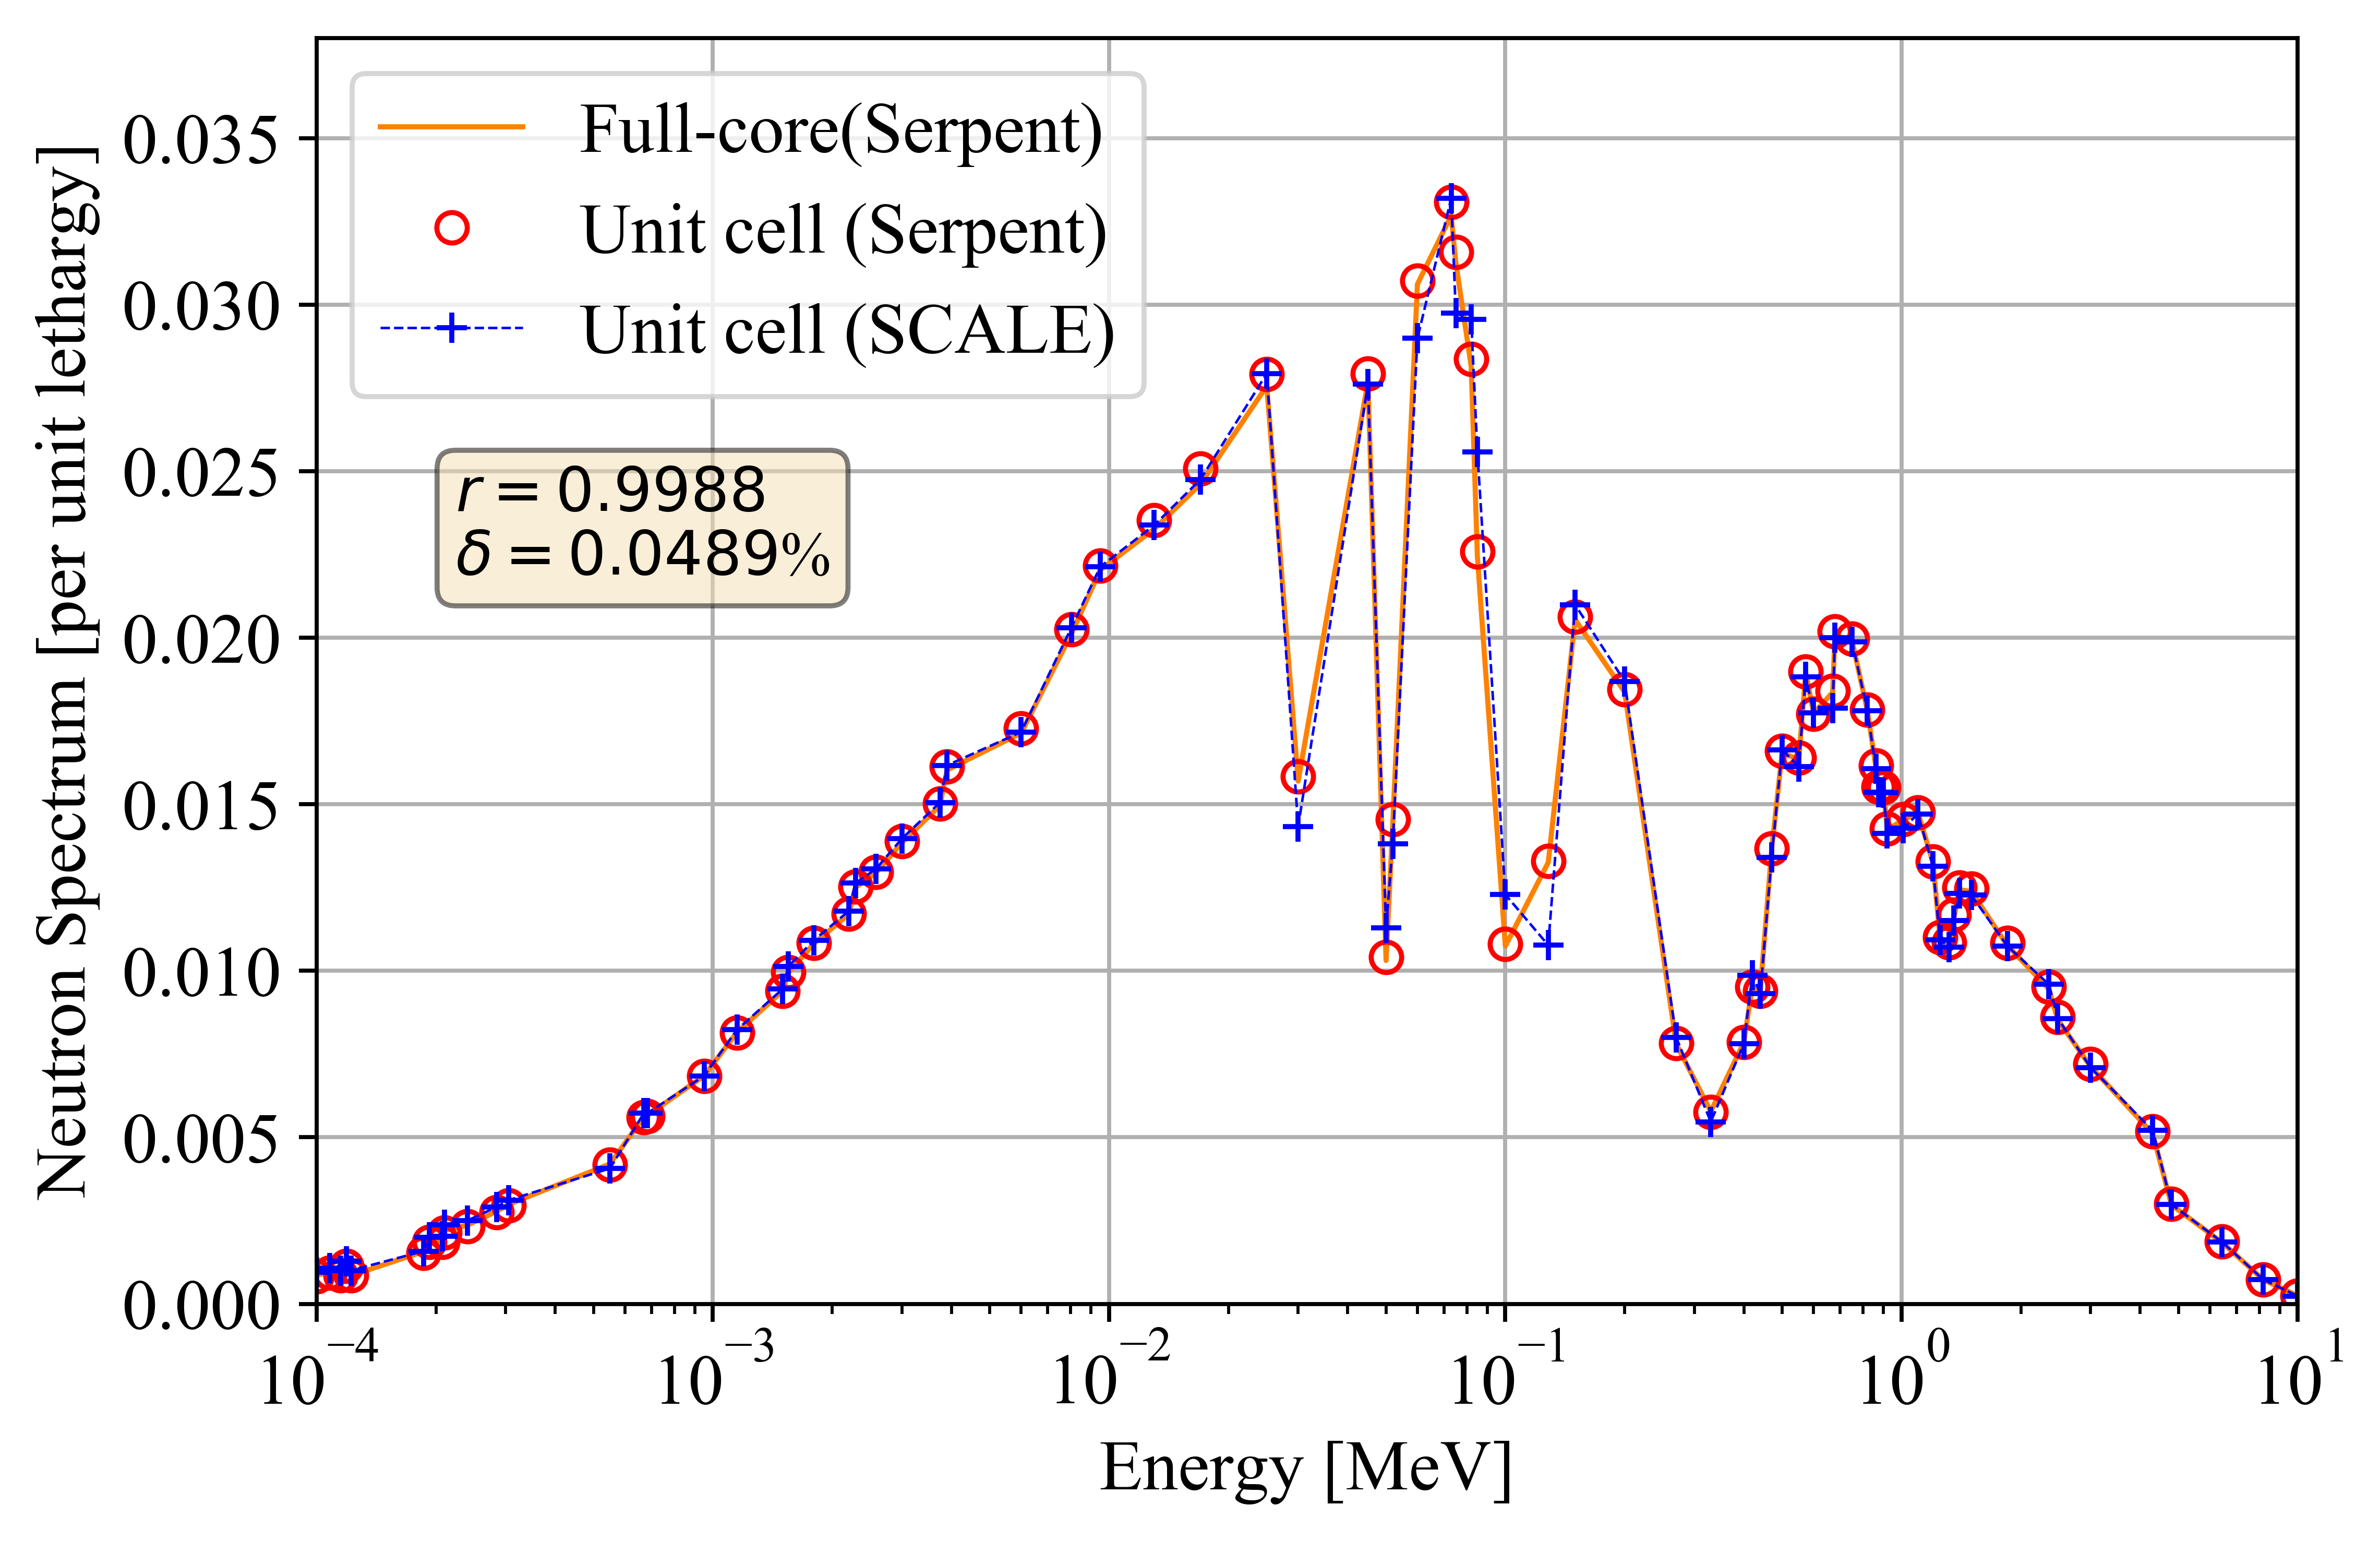
\includegraphics[scale=0.585]{./Figures/msfr_full_vs_unit_spectrum.png}
  \caption{Neutron flux energy spectrum for full-core and unit cell models for two-fluid \gls{MSFR}.}   
  \label{fig:spectrum_msfr}
\end{figure}
\begin{figure}[!htb]
  \centering
  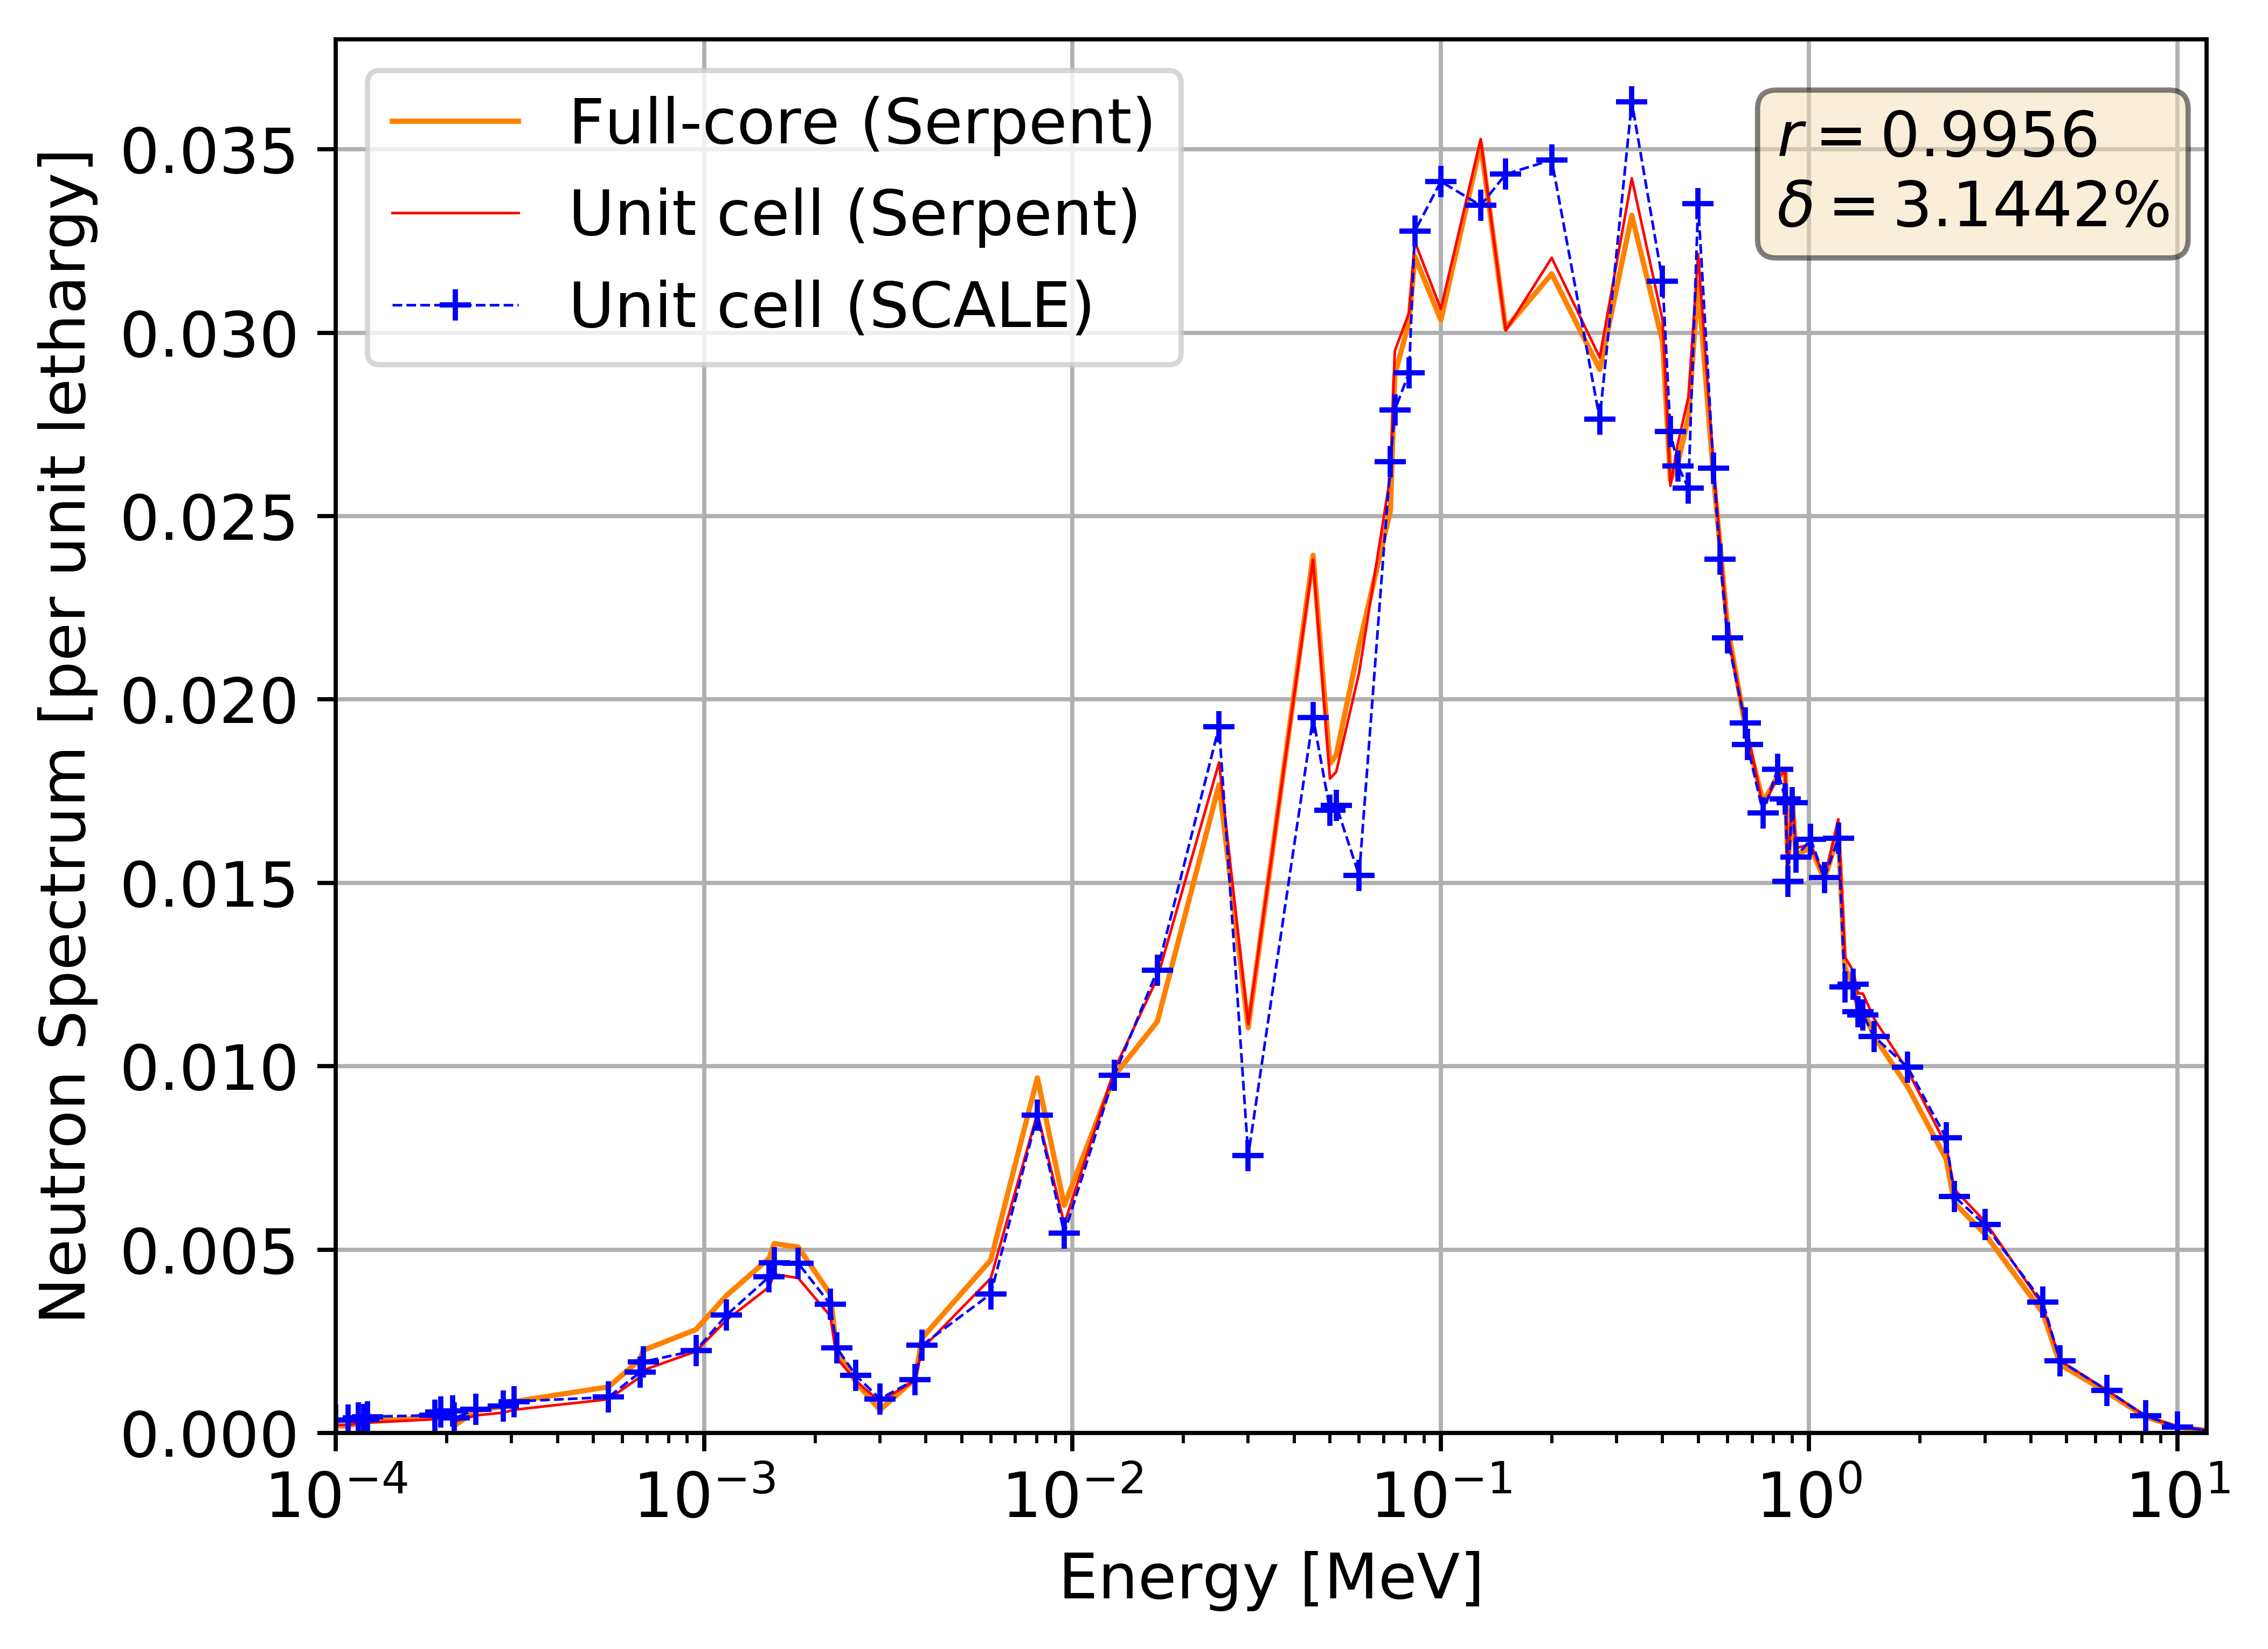
\includegraphics[scale=0.585]{./Figures/mcsfr_full_vs_unit_spectrum.png}
  \caption{Neutron flux energy spectrum for full-core and unit cell models for two-fluid \gls{MCSFR}.}   
  \label{fig:spectrum_mcsfr}
\end{figure}
\begin{figure}[!htb]
  \centering
  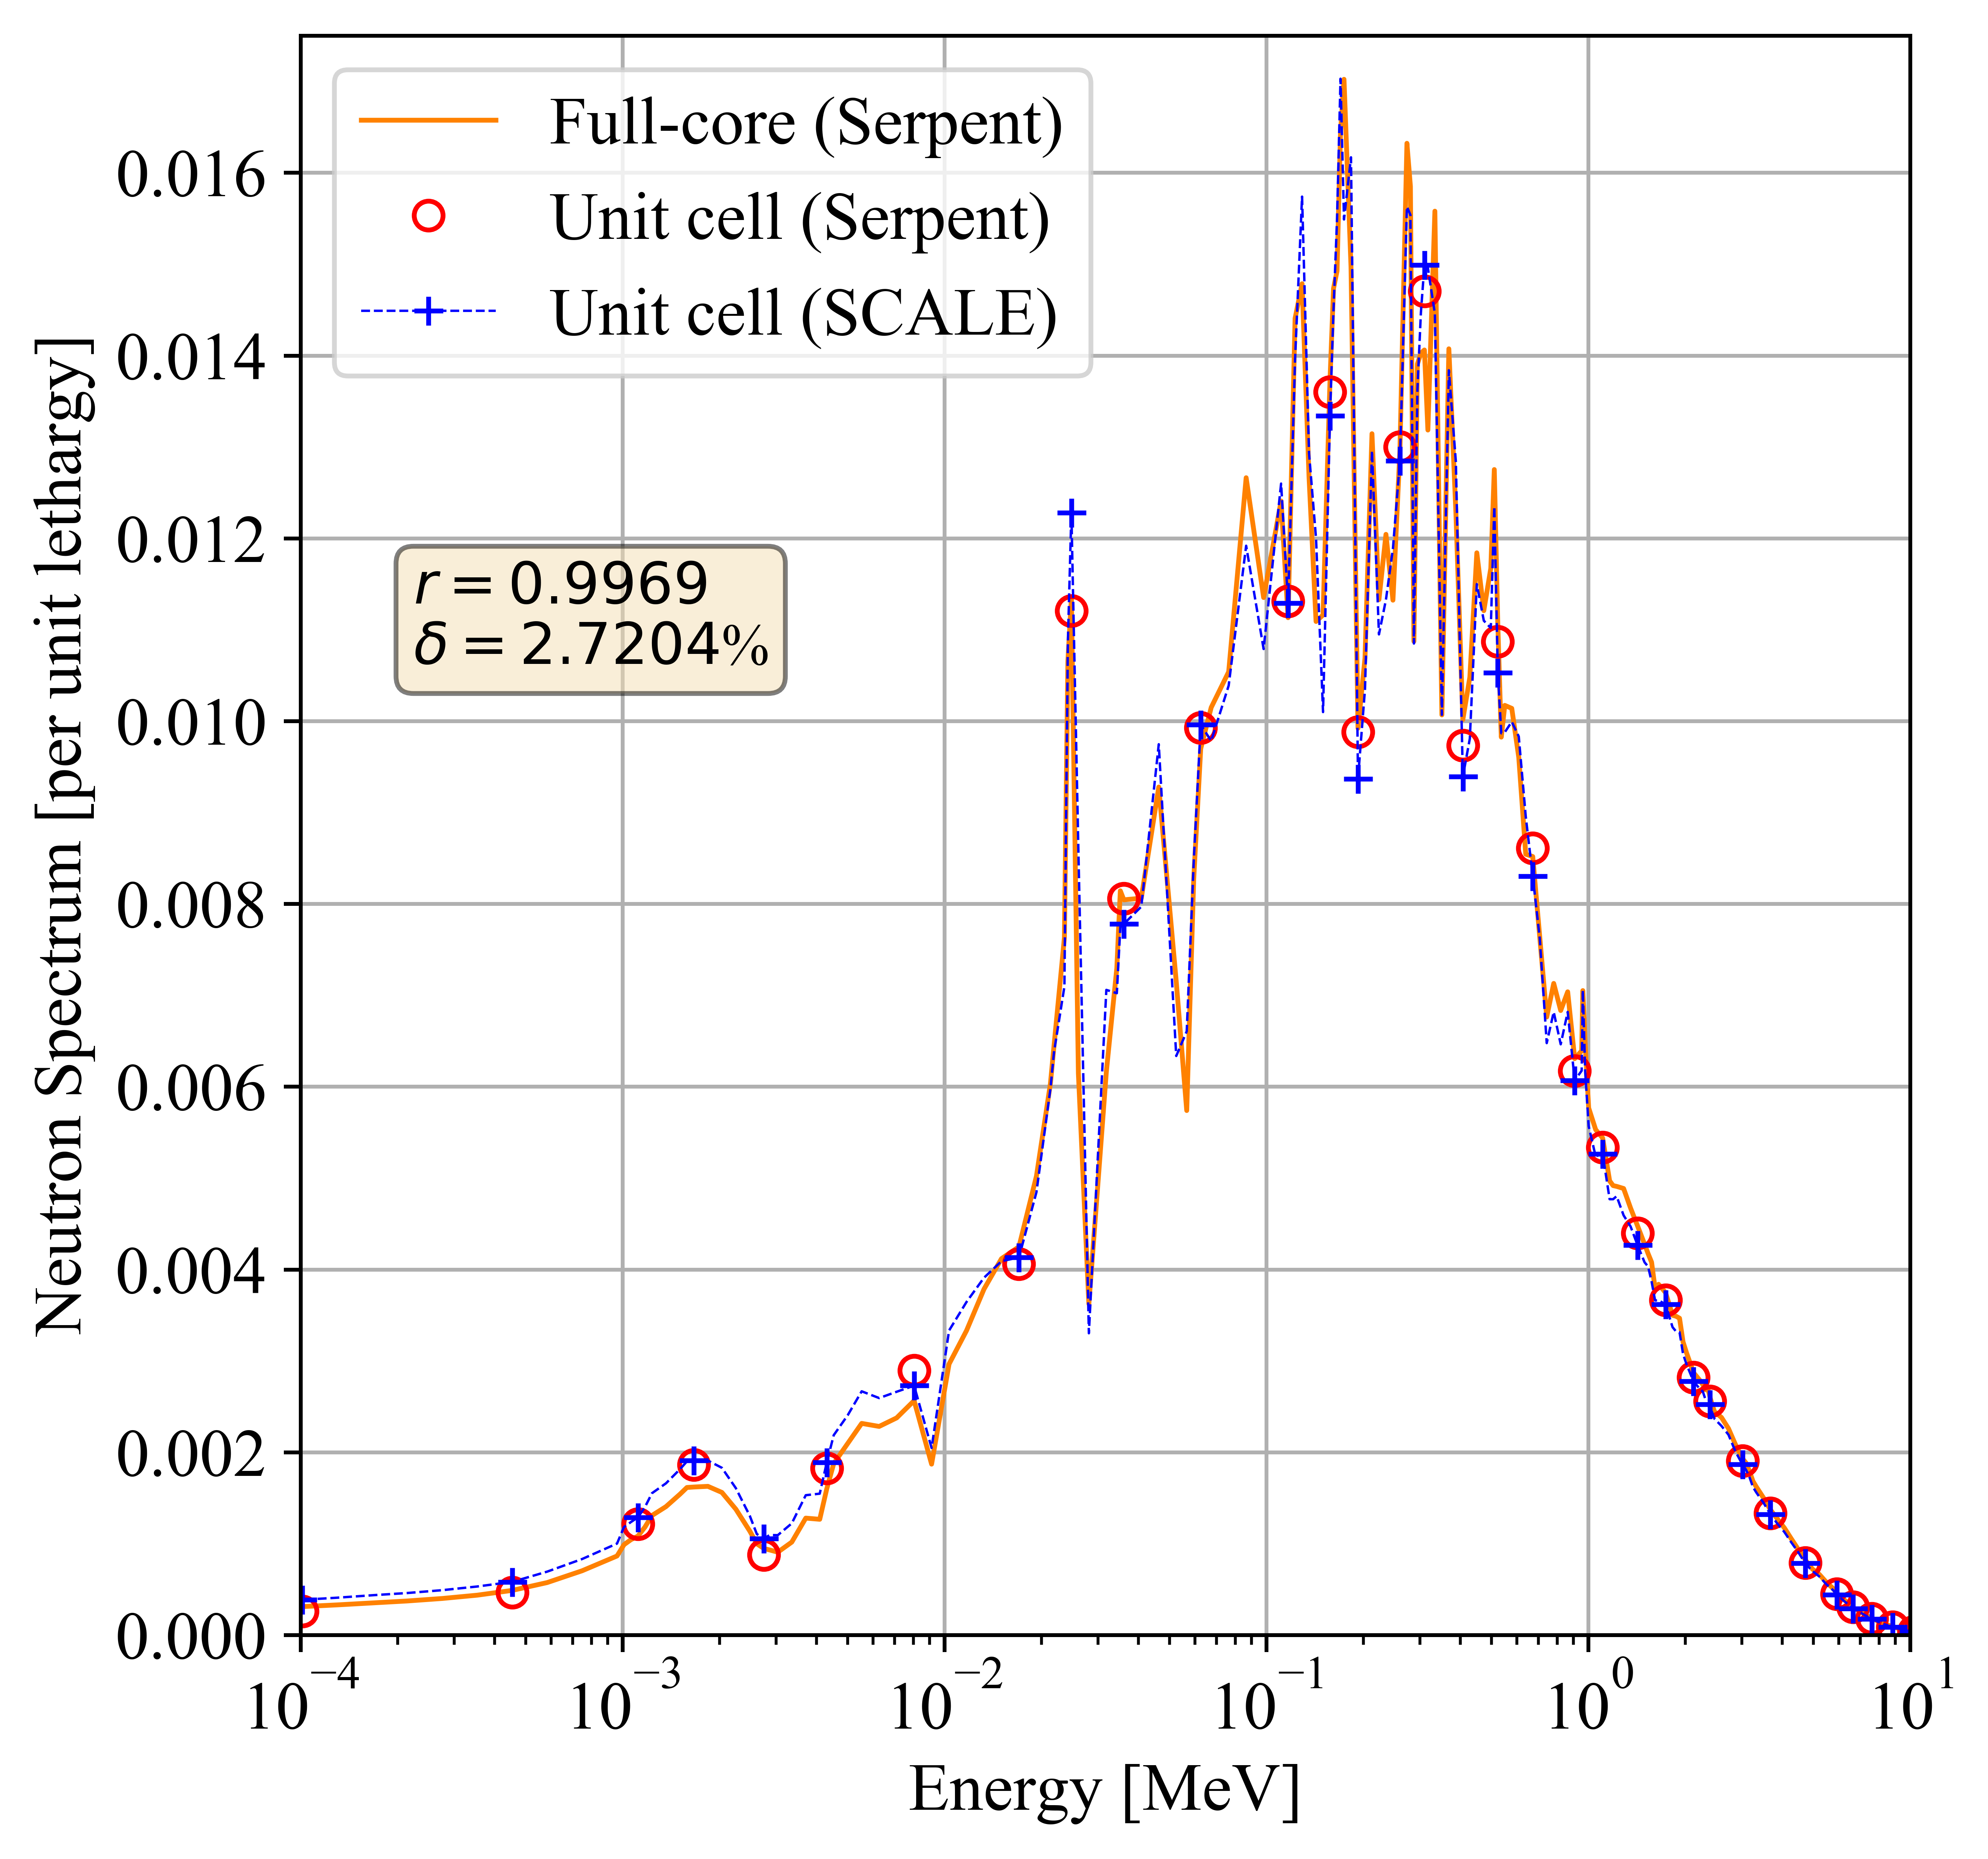
\includegraphics[scale=0.585]{./Figures/rebus_full_vs_unit_spectrum.png}
  \caption{Neutron flux energy spectrum for full-core and unit cell models for single-fluid REBUS-3700.}   
  \label{fig:spectrum_rebus}
\end{figure}
\begin{figure}[!htb]
  \centering
  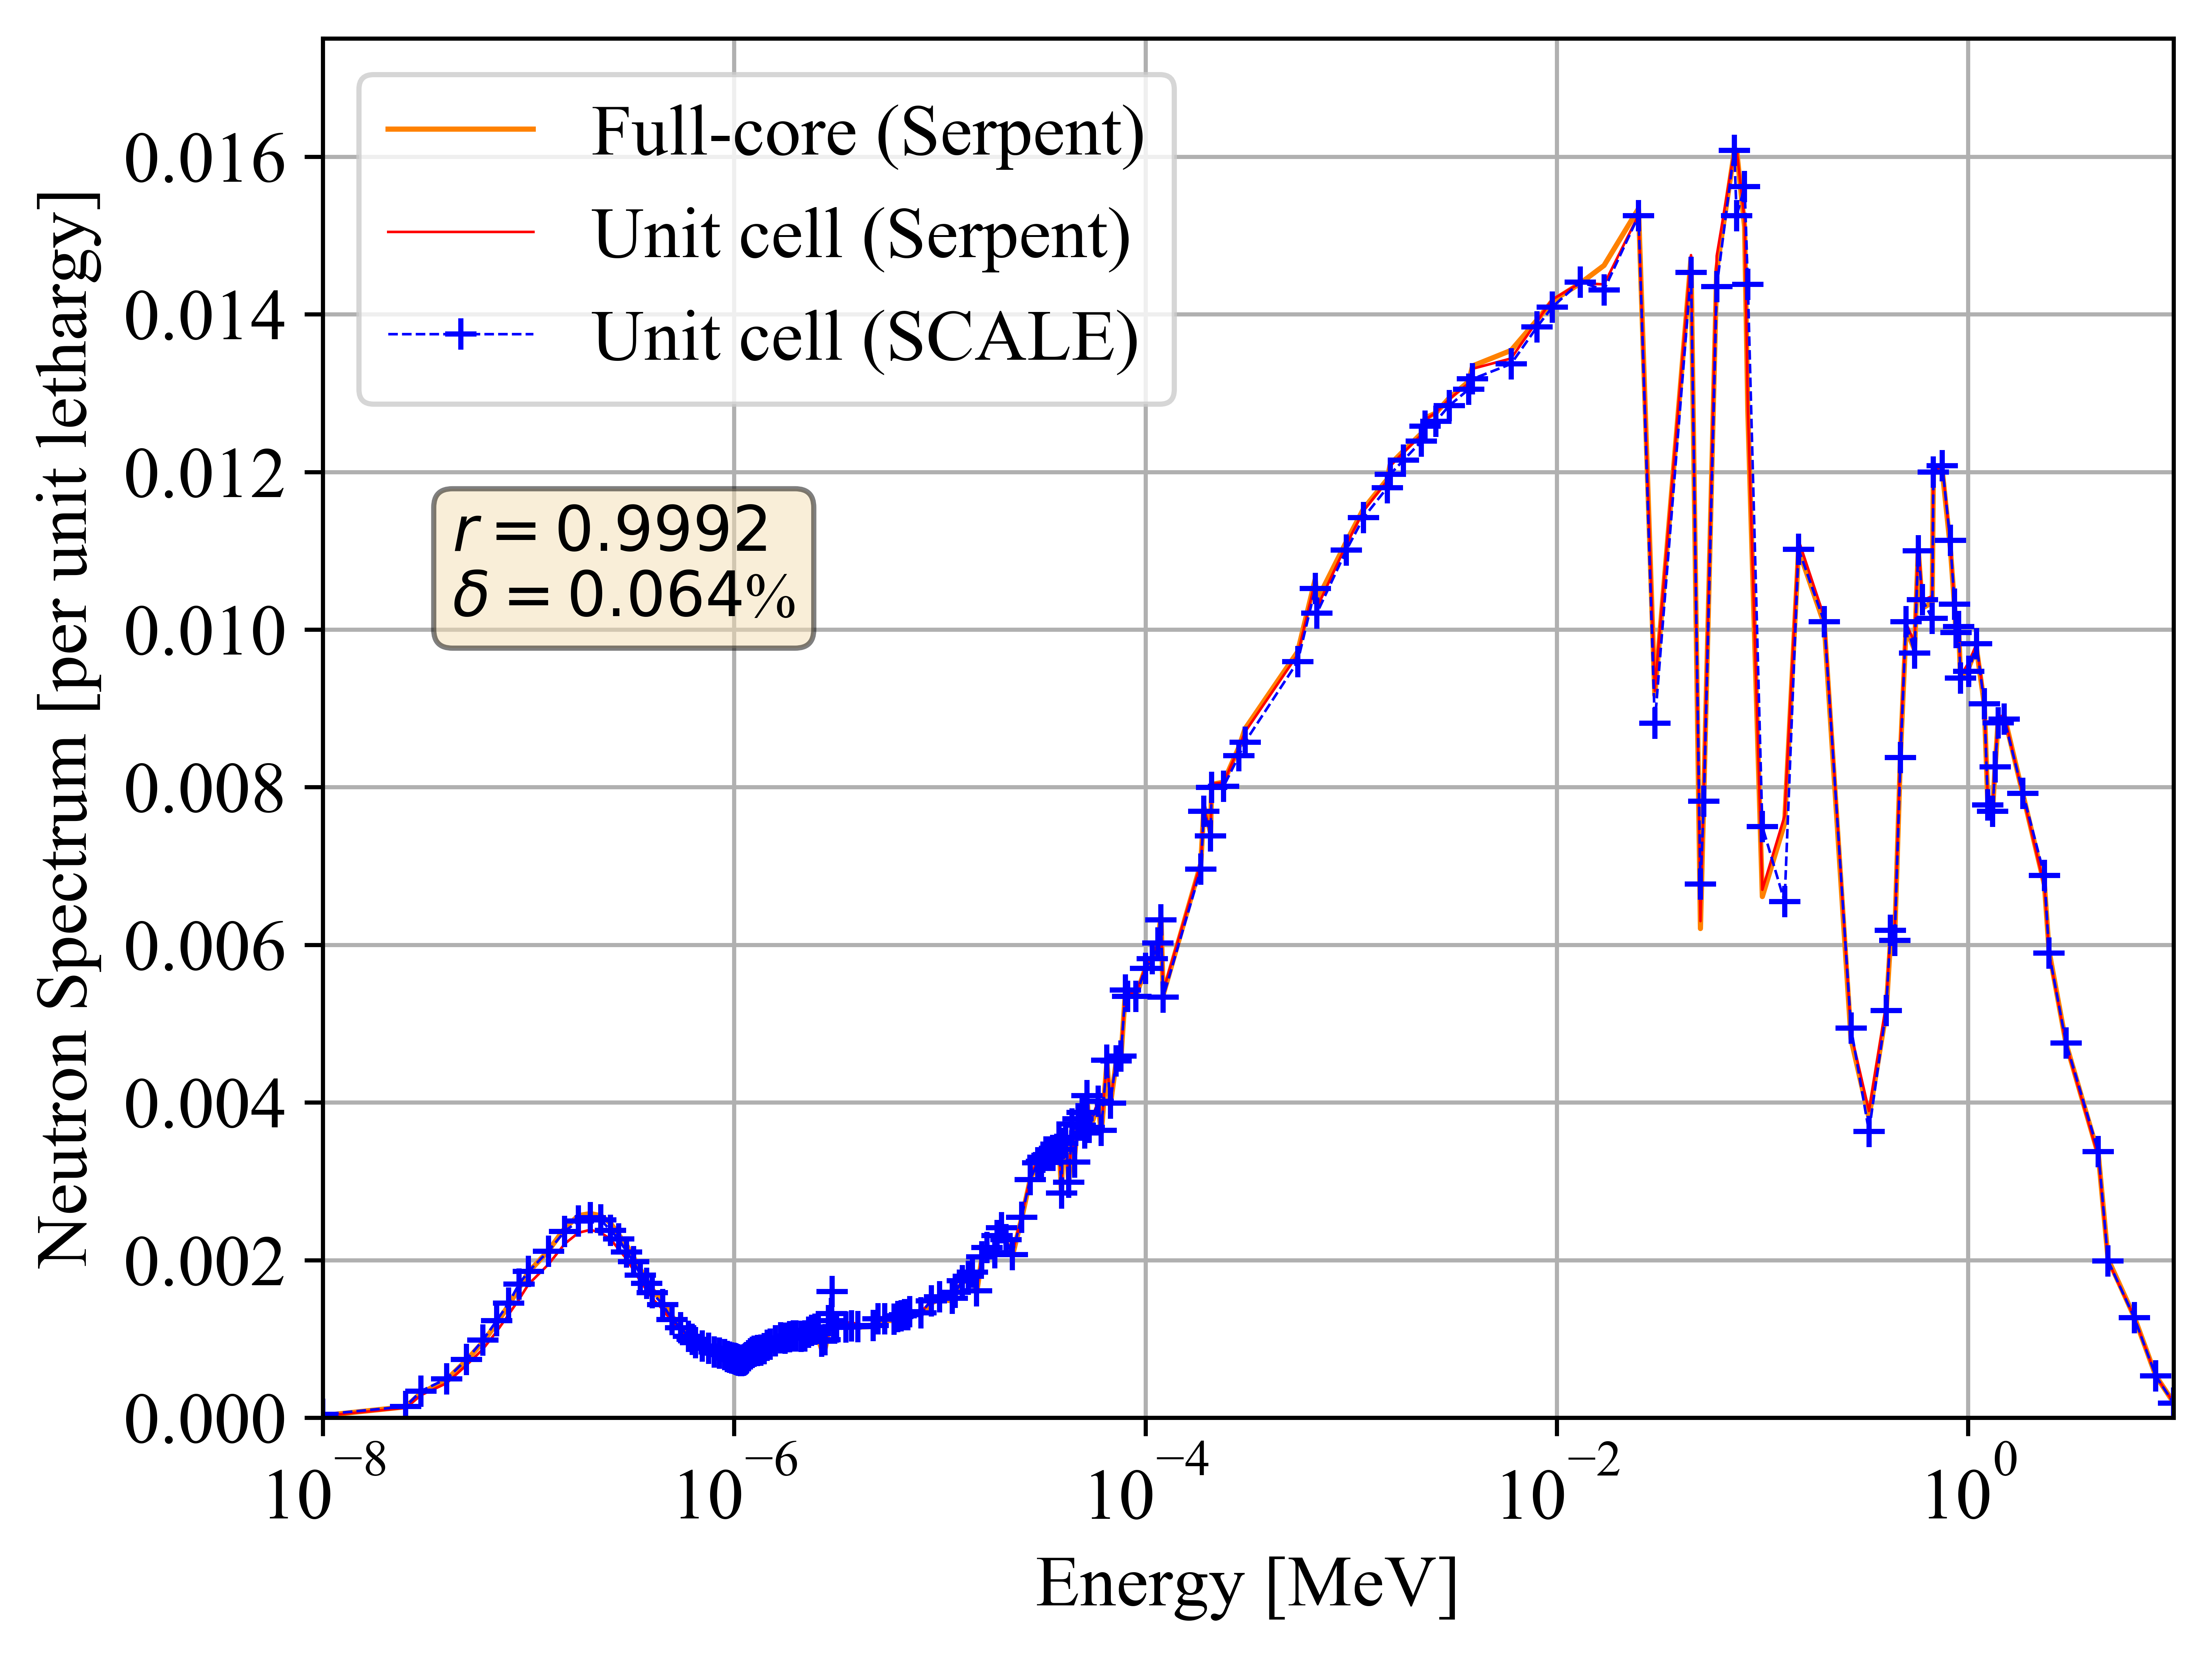
\includegraphics[scale=0.585]{./Figures/mosart_full_vs_unit_spectrum.png}
  \caption{Neutron flux energy spectrum for full-core and unit cell models for single-fluid \gls{MOSART} with graphite reflector.}   
  \label{fig:spectrum_mosart}
\end{figure}

When importing figures or any graphical image please verify two things:
\begin{itemize} \itemsep1pt \parskip0pt \parsep0pt
\item Any number, text or symbol is in Times font and is not smaller than 
  10-point after reduction to the actual window in your paper
\item That it can be translated into PDF
\end{itemize}

Equations, such as Eq. (\ref{sample_equation}), should be centered and 
sequentially numbered to the flush right of the formula.

\begin{equation}
  \label{sample_equation}
  \mathrm{Speedup}=\frac{1}{\frac{f}{p}+(1-f)}
\end{equation}

The continuation of a paragraph after an equation should not be indented.  
All paragraphs, as well as section or subsection headings, are separated by 
just one single empty line.

\subsubsection{Sub-subsection level and lower: only first character uppercase}

See Table \ref{table:example} for a sample table.  The ``tabls'' package is
recommended for improved row and column spacing.  Notice the caption appears 
above the table by setting the \verb!\caption! command immediately 
after the \verb!\begin{table}!. Tables are numbered in Roman 
numerals, with the caption centered above the table, in \textbf{boldface}.  
Triple-space before and after the table.

\begin{table}[!htb]
  \centering
  \caption{\bf Parallel Performance for the Sample Problem}
  \label{table:example} 
  \begin{tabular}{|c|c|c|c|} \hline 
   Parameter \\ \gls{MSFR} & (T$_{s}$/T$_{p}$) & (\%) \\ \hline
    \ 1 &  100.0 & \ ---    & ---  \\ \hline
    \ 2 &   52.6 & \ 1.9    & 95.0 \\ \hline 
  \end{tabular}
\end{table}

\section{CONCLUSIONS}

Present your summary and conclusions here.
%%%%%%%%%%%%%%%%%%%%%%%%%%%%%%%%%%%%%%%%%%%%%%%%%%%%%%%%%%%%%%%%%%%%%%%%%%%%%%%%
\section{Acknowledgments}
This research was supported by the Fuel Cycles Options Campaign of the Fuel Cycle Technologies initiative 
and by an appointment to the Oak Ridge National Laboratory Nuclear Engineering Science Laboratory Synthesis (NESLS) Program, sponsored by U.S. Department of Energy and administered by the Oak Ridge Institute for Science and Education.

%%%%%%%%%%%%%%%%%%%%%%%%%%%%%%%%%%%%%%%%%%%%%%%%%%%%%%%%%%%%%%%%%%%%%%%%%%%%%%%%
\bibliographystyle{ans}
\bibliography{2019-rykh-fsmsrs-mc}
\end{document}

